\section{玻恩近似}


\begin{quotation}
“我在思维的飞跃中找到了自己的乐趣,而并不太喜欢用严密的逻辑推理来进行论证。”\qquad 汤川秀树
\end{quotation}



如果入射粒子能量(对应$H_0  = {{p^2 } \mathord{\left/
 {\vphantom {{p^2 } {2m}}} \right.
 \kern-\nulldelimiterspace} {2m}}$)较大, 分波法计算将变得极为冗长, 这时,我们可尝试把入射粒子与散射中心的相互作用(对应$H' = V(r)$)当作微扰处理,这种方法就是玻恩近似。


\subsection{玻恩近似}

\index{Born approximation: 玻恩近似}

$H_0  = {{p^2 } \mathord{\left/
 {\vphantom {{p^2 } {2m}}} \right.
 \kern-\nulldelimiterspace} {2m}}$
对应的解是平面波$\psi _k  = \frac{1}{{\sqrt V }}e^{ik \cdot r} $;$H' = V(r)$是短程力,所以入射波函数($r \to  - \infty $),散射波函数($r \to \infty $)都可用平面波表示。

假设:$\psi _i  = \frac{1}{{\sqrt V }}e^{ik_i  \cdot r} $(入射波函数);$\psi _f  = \frac{1}{{\sqrt V }}e^{ik_f  \cdot r} $(散射波函数),$k_f$在$\left( {\theta ,\varphi } \right)$方向上;


入射粒子流密度:$j_i  = \frac{{i\hbar }}{{2m}}\left( {\psi \nabla \psi ^*  - \psi ^* \nabla \psi } \right) = \frac{1}{V}\frac{{\hbar k_i }}{m} = \frac{{v_i }}{V}$

根据散射截面定义,单位时间有$dn$个粒子散射到$\left( {\theta ,\varphi } \right)$方向:

\begin{equation}\label{27-1}
dn = \sigma \left( {\theta ,\varphi } \right)j_i d\Omega  = \sigma \left( {\theta ,\varphi } \right)\frac{{v_i }}{V}d\Omega
\end{equation}


\index{Fermi's golden rule: 费米黄金规则}

根据费米黄金规则:$w_{fi}  = \frac{{2\pi }}{\hbar }\left| {H'_{fi} } \right|^2 \rho (E_f )$


单位时间散射到$\left( {\theta ,\varphi } \right)$方向的几率是:


\begin{equation}\label{27-2}
dn = w_{fi}  = \frac{{2\pi }}{\hbar }\left| {\left\langle {f\left| {H'} \right|\left. i \right\rangle } \right.} \right|^2 \rho \left( {E_f } \right)
\end{equation}

\index{Density of states: 态密度}

$\rho \left( {E_f } \right)$是散射粒子(末态)的态密度\footnote{态密度的计算:

$dN = \frac{1}{{h^3 }}dxdydzdp_x dp_y dp_z $, $p \to p + dp$内的状态数:$dN = \frac{V}{{h^3 }}dp_x dp_y dp_z $

由直角坐标系变为球坐标系:$dp_x dp_y dp_z  \to p^2 dp\sin \theta d\theta d\varphi $

$dN = \frac{V}{{h^3 }}p^2 dp\sin \theta d\theta d\varphi =
\frac{V}{{h^3 }}p^2 dpd\Omega $; $E_f  = \frac{{p_f^2 }}{{2m}}$,
$dE_f  = \frac{{p_f }}{m}dp_f $; 所以: $\rho \left( {E_f } \right) =
\frac{{dN}}{{dE_f }} = \frac{V}{{h^3 }}mp_f d\Omega $};

\begin{equation}\label{27-3}
\rho \left( {E_f } \right) = \frac{{dN}}{{dE_f }} = \frac{V}{{h^3 }}mp_f d\Omega
\end{equation}


所以:$\sigma \left( {\theta ,\varphi } \right)\frac{{v_i }}{V}d\Omega  = \frac{{2\pi V}}{{\hbar h^3 }}\left| {\left\langle {f\left| {H'} \right|\left. i \right\rangle } \right.} \right|^2 mp_f d\Omega $


\begin{equation}\label{27-4}
\sigma \left( {\theta ,\varphi } \right) = \frac{{2\pi m^2 V^2 }}{{\hbar h^3 }}\frac{{v_f }}{{v_i }}\left| {\left\langle {f\left| {H'} \right|\left. i \right\rangle } \right.} \right|^2
\end{equation}


其中:$\left| {\left\langle {f\left| {H'} \right|\left. i \right\rangle } \right.} \right|^2  = \left| {\frac{1}{V}\int {d^3 rV(r)e^{i\left( {k_i  - k_f } \right) \cdot r} } } \right|^2  = \frac{1}{{V^2 }}\left| {V(k_i  - k_f )} \right|^2 $

所以:$\sigma \left( {\theta ,\varphi } \right) = \frac{{2\pi m^2 V^2 }}{{\hbar h^3 }}\frac{{v_f }}{{v_i }}\left| {\left\langle {f\left| {H'} \right|\left. i \right\rangle } \right.} \right|^2  = \frac{{2\pi m^2 }}{{\hbar h^3 }}\frac{{v_f }}{{v_i }}\left| {V(k_i  - k_f )} \right|^2 $


根据弹性散射条件:$k_f = k_i$, $v_f = v_i$, 所以:


\begin{equation}\label{27-5}
\sigma \left( \theta  \right) = \frac{{2\pi m^2 }}{{\hbar h^3 }}\left| {V(k_i  - k_f )} \right|^2
\end{equation}

令:$\mathord{\buildrel{\lower3pt\hbox{$\scriptscriptstyle\rightharpoonup$}}
\over k} _f  - \mathord{\buildrel{\lower3pt\hbox{$\scriptscriptstyle\rightharpoonup$}}
\over k} _i  = \mathord{\buildrel{\lower3pt\hbox{$\scriptscriptstyle\rightharpoonup$}}
\over q} $,$q = 2k\sin {\textstyle{\theta  \over 2}}$,取$\vec q$方向为极轴方向;


$\begin{array}{l}
 V(k_i  - k_f ) = \int {d^3 rV(r)e^{ - iq \cdot r} }  \\
 = \int_0^\infty  {V(r)r^2 dr} \int_0^\pi  {e^{ - iqr\cos \theta } \sin \theta d\theta } \int_0^{2\pi } {d\varphi }  \\
  = 2\pi \int_0^\infty  {V(r)r^2 dr} \int_0^\pi  {e^{ - iqr\cos \theta } d\left( { - \cos \theta } \right)}  \\
  = 2\pi \int_0^\infty  {V(r)r^2 dr}  \times \left[ {\frac{{e^{iqr}  - e^{ - iqr} }}{{iqr}}} \right] \\
  = \frac{{4\pi }}{q}\int_0^\infty  {\sin qrV(r)rdr}  \\
 \end{array}$


所以:

\begin{equation}\label{27-6}
\begin{array}{l}
 \sigma \left( \theta  \right) = \frac{{2\pi m^2 }}{{\hbar h^3 }}\left| {\frac{{4\pi }}{q}\int_0^\infty  {\sin qrV(r)rdr} } \right|^2  = \frac{{2\pi m^2 }}{{\hbar h^3 }}\frac{{16\pi ^2 }}{{q^2 }}\left| {\int_0^\infty  {\sin qrV(r)rdr} } \right|^2  \\
  = \frac{{4m^2 }}{{\hbar ^4 q^2 }}\left| {\int_0^\infty  {\sin (qr)V(r)rdr} } \right|^2  \\
 \end{array}
\end{equation}


\subsection{玻恩近似成立的条件}

只有在散射势可以被看作微扰时,玻恩近似才成立。或说:考虑微扰后波函数$\psi  = \psi _i  + \psi _s $
偏离$\psi_i$不大时近似成立。首先,玻恩近似不适用长程力,如库仑场,因为在受长程力散射时,即使粒子离散射中心很远,$\psi$ 就已经不能被当作平面波处理,由于作用力程较长,对波函数累积的效果可能会很大,如库仑场($V(r) \sim \frac{1}{r}$),会导致积分不收敛。

对于短程力,我们使用力程:$a$,平均势:$\bar V$来表征,即:

\begin{equation}\label{27-7}
\left\{ \begin{array}{l}
 V(r) = \bar V,r \le a \\
 V(r) = 0,r > a \\
 \end{array} \right.
\end{equation}


如果$\psi$偏离$\psi_i$(平面波)不大,在力程以内, 波函数发生变形,
但仍可近似看作是``平面波'', 具有近似确定的动量,即:$\Delta p \ll
\frac{\hbar }{a}$;根据能量守恒,在力程以内,粒子动能改变为$\Delta
E_k  \sim \bar V$量级。即:$\bar V \sim \Delta E_k  = \Delta \left(
{\frac{{p^2 }}{{2m}}} \right) = \frac{p}{m}\Delta p \ll \frac{p}{m}
\cdot \frac{\hbar }{a}$

所以:$\frac{{ma\bar V}}{{\hbar p}} \ll 1$, 由于$p = mv$


所以玻恩近似适用条件: $\frac{{a\bar V}}{{\hbar v}} \ll
1$,即适用于粒子的高能散射\footnote{参考蔡建华《量子力学
上册》第162页; 曾谨言《量子力学 卷I》第687页}。

\subsection{屏蔽库仑场散射}



库仑力:$V(r) =  - \frac{{Z_1 Z_2 e^2 }}{{4\pi \varepsilon _0
r}}$是长程力, 如果直接代入公式:$\sigma (\theta ) = \frac{{4m^2
}}{{\hbar ^4 q^2 }}\left| {\int_0^\infty  {\sin (qr)V(r)rdr} }
\right|^2 $ 计算,积分:

$\int_0^\infty  {\sin (qr)V(r)rdr}  =  -
\frac{{Z_1 Z_2 e^2 }}{{4\pi \varepsilon _0 }}\int_0^\infty  {\sin
(qr)} dr$不收敛。



实际原子核所产生电场被原子内部电子所屏蔽, 屏蔽库仑场是短程力:

\index{Screened Coulomb potential: 屏蔽库仑势}

\begin{equation}\label{screened coulomb potential}
V(r) = - \frac{{Z_1 Z_2 e^2 }}{{4\pi \varepsilon _0 r}}e^{ - \alpha
r}
\end{equation}


在 $r \sim {1 \mathord{\left/
 {\vphantom {1 \alpha }} \right.
 \kern-\nulldelimiterspace} \alpha }$ 尺度(屏蔽半径或力程)内, 屏蔽库仑场作用明显, 否则会很快衰减掉。



$\begin{array}{l}
 \sigma (\theta ) = \frac{{4m^2 }}{{\hbar ^4 q^2 }}\left| {\int_0^\infty  {\sin (qr)V(r)rdr} } \right|^2  = \frac{{4m^2 }}{{\hbar ^4 q^2 }}\left| {\int_0^\infty  {\sin (qr)\frac{{Z_1 Z_2 e^2 }}{{4\pi \varepsilon _0 }}e^{ - \alpha r} dr} } \right|^2  \\
  = \frac{{4m^2 }}{{\hbar ^4 q^2 }}\left( {\frac{{Z_1 Z_2 e^2 }}{{4\pi \varepsilon _0 }}} \right)^2 \left| {\int_0^\infty  {\sin (qr)e^{ - \alpha r} dr} } \right|^2  \\
 \end{array}$


其中积分:

$\begin{array}{l}
 \int_0^\infty  {\sin (qr)e^{ - \alpha r} dr}  = \int_0^\infty  {\frac{{e^{iqr}  - e^{ - iqr} }}{{2i}}} e^{ - \alpha r} dr = \frac{1}{{2i}}\int_0^\infty  {\left( {e^{(iq - \alpha )r}  - e^{ - (iq + \alpha )r} } \right)} dr \\
  = \frac{1}{{2i}}\left[ {\frac{{e^{(iq - \alpha )r} }}{{iq - \alpha }} + \frac{{e^{ - (iq + \alpha )r} }}{{iq + \alpha }}} \right]_0^\infty   =  - \frac{1}{{2i}}\left[ {\frac{1}{{iq - \alpha }} + \frac{1}{{iq + \alpha }}} \right] =  - \frac{1}{{2i}}\frac{{2iq}}{{\left( {iq - \alpha } \right)\left( {iq + \alpha } \right)}} \\
  = \frac{q}{{q^2  + \alpha ^2 }} \\
 \end{array}$

所以:$\sigma (\theta ) = \frac{{4m^2 }}{{\hbar ^4 q^2 }}\left( {\frac{{Z_1 Z_2 e^2 }}{{4\pi \varepsilon _0 }}} \right)^2 \left| {\frac{q}{{q^2  + \alpha ^2 }}} \right|^2  = \frac{{4m^2 }}{{\hbar ^4 }}\left( {\frac{{Z_1 Z_2 e^2 }}{{4\pi \varepsilon _0 }}} \right)^2 \frac{1}{{\left( {q^2  + \alpha ^2 } \right)^2 }}$


库仑场条件下:$\alpha  \to 0$,得到卢瑟福散射公式,

\index{Rutherford scattering: 卢瑟福散射}

\begin{equation}\label{27-8}
\begin{array}{c}
\sigma (\theta ) = \frac{{4m^2 }}{{\hbar ^4 }}\left( {\frac{{Z_1 Z_2
e^2 }}{{4\pi \varepsilon _0 }}} \right)^2 \frac{1}{{q^4 }} =
\frac{{4m^2 }}{{\hbar ^4 }}\left( {\frac{{Z_1 Z_2 e^2 }}{{4\pi
\varepsilon _0 }}} \right)^2 \frac{1}{{16k^4 \sin ^4
{\textstyle{\theta  \over 2}}}} \\
 = \frac{{Z_1 ^2 Z_2 ^2 }}{{16E_k ^2
}}\left( {\frac{{e^2 }}{{4\pi \varepsilon _0 }}} \right)^2
\frac{1}{{\sin ^4 {\textstyle{\theta  \over 2}}}} \\
\end{array}
\end{equation}


定义:$a = \frac{{Z_1 Z_2 e^2 }}{{4\pi \varepsilon _0 E_k }}$,则:$\sigma (\theta ) = \left( {\frac{a}{4}} \right)^2 \frac{1}{{\sin ^4 {\textstyle{\theta  \over 2}}}}$

\index{Coulomb Scattering: 库仑散射}

库仑场是长程力, 玻恩近似原则上是不适用于库仑散射的,
但按屏蔽库仑场在``屏蔽''距离为无穷大时所得到的散射截面公式与经典力学解相同,
与量子力学的严格解也完全相同。这究竟是个偶然巧合, 还是有其内在原因,
目前尚无定论。


\begin{figure}[h]
\begin{center}
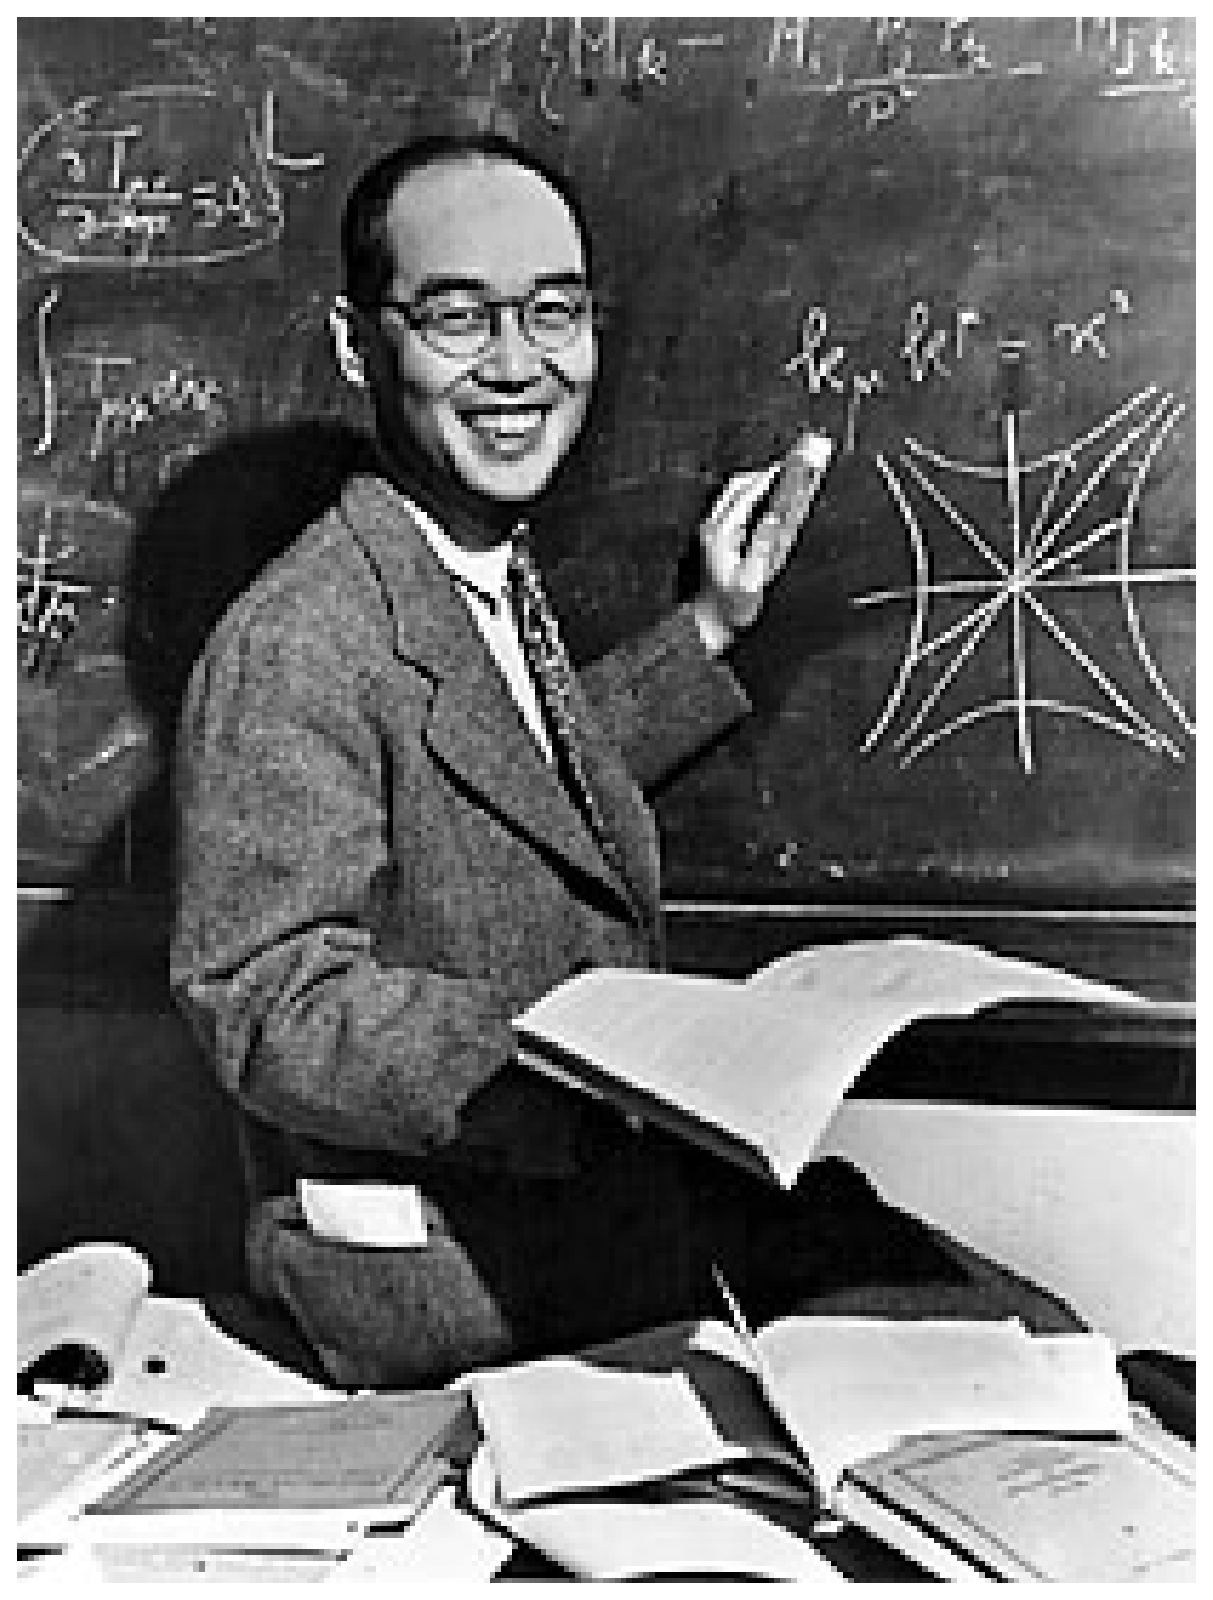
\includegraphics[clip,width=5cm]{Scattering/yukawa.ps}
\caption{汤川秀树}
\end{center}
\end{figure}



\subsection*{阅读与思考}


\index{Yukawa potential: 汤川势}

屏蔽库仑势\ref{screened coulomb potential},
也叫\textbf{汤川势}(Yukawa potential)。汤川秀树(Hideki
Yukawa)提出核子(nucleon)是``介子场''(meson field)的``源'',
介子质量对应$\alpha$, 类比电磁相互作用中, 电荷(chanrge)是静电场的源,
传播电磁场的光子的静质量为$0$。对静电场而言, $\alpha = 0$,
力程无穷远。核力是短程力, 力程: $\sim \frac{1}{\alpha}$,
汤川估计$\alpha \sim 200 m_e$, 实验观测值$\sim 270 m_e$(Powell,
1947年数据)。

\index{photon: 光子}


更多请阅读:J. J. Sakurai, \textbf{Advanced Quantum Mechanics},
第一章。

汤川秀树是第一个获得诺贝尔奖的东亚人(1949),而且他的教育和研究主要都是在日本本土完成的,汤川在日本国内完成的关于介子的工作使他的同学,当时(二战前)正在德国师从海森堡研究量子力学的朝永振一郎颇感郁闷。最终朝永因他在量子场论中的工作在1965年与费曼和施温格分享了诺贝尔物理奖。

关于汤川秀树,可阅读:《创造力与直觉》、《旅人:一个物理学家的回忆》。







